%! Author = Len Washington III
%! Date = 8/12/2023

% Preamble
\documentclass[12pt]{report}

% Packages
\usepackage[7]{cs430homework}

% Document
\begin{document}

\maketitle

\begin{enumerate}[label=\arabic*.]
	\item (5 points) The \textbf{clustering coefficient} $C(G)$\label{def:cg} of a simple graph G is the probability that if $u$ and $v$ are neighbors and $v$ and $w$ are neighbors, then $u$ and $w$ are neighbors, where $u$, $v$, and $w$ are distinct vertices of $G$.
	\begin{enumerate}[label=\arabic{enumi}\alph*)]
	    \item We say that three vertices $u$, $v$, and $w$ of a simple graph $G$ form a triangle if there are edges connecting all three pairs of these vertices. Find a formula for \hyperref[def:cg]{$C(G)$} in terms of the number of triangles in $G$ and the number of paths of length two in the graph. [Hint: Count each triangle in the graph once for each order of three vertices that form it.]
		\item Explain what the clustering coefficient measures in each of these graphs.
		\begin{itemize}
			\item the Hollywood graph (used for the six degrees of Kevin Bacon problem)
			\item the graph of Facebook friends
			\item the graph representing the routers and communications links that make up the worldwide Internet
		\end{itemize}
	\end{enumerate}
	\item (5 points) Let $G$ be a directed graph represented using an adjacency list. So, each node $G[i]$ has a list of all nodes reachable in 1 step from $i$ (all out-neighbors of $i$). Suppose each node of $G$ also has a value: e.g., node 1 might have value \$100, node 2 might have value \$50, etc.\\
	Give an $O(|E| + |V | \log |V |)$ time algorithm that computes, for every node, the highest value reachable from that node (i.e., that you can get to by some path from that node). For instance, if it is possible to get to any node from any other node ($G$ is “strongly-connected”), then for every node this will be the maximum value in the entire graph. Hint: one worthwhile preprocessing step is to sort nodes by value.
	\item (5 points) Suppose you are implementing a spreadsheet program, in which you must maintain a grid of cells (each designated by alphabetic row and integer column). Some cells of the spreadsheet contain numbers, but other cells contain expressions that depend on other cells for their value. However, the expressions are not allowed to have a circular reference: for example, if the expression in cell $E1$ depends on the value of cell $A5$, and the expression in cell $A5$ depends on the value of cell $C2$, then $C2$ must not depend on $E1$.
	\begin{enumerate}[label=\arabic{enumi}\alph*)]
	    \item Describe an efficient algorithm for making sure that no circular reference exists (or finding one and complaining to the spreadsheet user if it does exist).
		\item If the spreadsheet changes, all its expressions may need to be recalculated. Describe an efficient method for sorting the expression evaluations, so that each cell is recalculated only after the cells it depends on have been recalculated.
	\end{enumerate}
	\item (5 points) For a sparse graph $G=\left\{V,E\right\}$, where $|E|=\Theta(V)$, is the implementation of Prim’s algorithm with a Fibonacci heap asymptotically faster than the binary-heap implementation? What about for a dense graph, $|E|=\Theta(V^{2})$? How must the sizes $|E|$ and $|V|$ be related for the Fibonacci-heap implementation to be asymptotically faster than the binary-heap implementation?
	\item (5 points) Prim’s and Kruskal’s algorithms both ``grow'' a minimum spanning tree of a graph by selecting edges to add to the tree in a specified, greedy order. Design an efficient algorithm to ``prune'' a graph and yield a minimum spanning tree by removing edges from the graph in a specified, greedy order. Prove optimal substructure and the Greedy Choice Property.
	\item (5 points) Let graph $G=\left(V,E\right)$ and vertices start, goal in $V$ be given. Assuming all edges in $E$ are of non-negative weight, describe an efficient algorithm for finding the longest acyclic path from start to goal.
	\item (5 points) A telephone network diagram is a weighted graph where the vertices represent switching centers and the edges represent lines between two centers. The edges are labeled by their bandwidth. We define the bandwidth of a path as the smallest bandwidth of an edge in the path. Give an algorithm that computes a path of maximum bandwidth between two given vertices of a telephone network diagram. For example, in the telephone network diagram shown below, $v_{1}v_{2}v_{4}$ is a path of maximum bandwidth (equal to 5) between vertices $v_{1}$ and $v_{4}$, and $v_{1}v_{2}v_{4}v_{3}$ is a path of maximum bandwidth (equal to 4) between vertices $v_{1}$ and $v_{4}$ \begin{figure}[H]
	\centering
	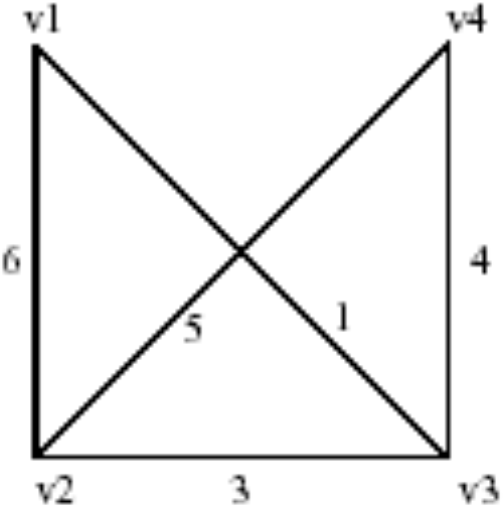
\includegraphics[width=0.5\textwidth]{7.7}
	\caption{}
	\label{fig:7}
\end{figure}

	\item (5 points) Suppose we also wish to compute the vertices on shortest paths in the algorithms of this section, instead of keeping track of the predecessors as we compute the shortest paths. Show how to compute the predecessor matrix $\Pi$ from the completed matrix $L$ of shortest-path weights in $O(n^{3})$ time.
\end{enumerate}

\end{document}